\chapter[Arquitetura]{Arquitetura}
\addcontentsline{toc}{chapter}{Arquitetura}

\section{Visão Geral}

A arquitetura do sistema é composta por três componentes principais: o servidor, o cliente e o banco de dados. O servidor é responsável por receber as requisições do cliente e enviar as respostas. O cliente é responsável por enviar as requisições ao servidor e receber as respostas. O banco de dados é responsável por armazenar os dados do sistema.

\subsection{Servidor}

O servidor é responsável por receber as requisições do cliente e enviar as respostas. O servidor é composto por um conjunto de módulos que são responsáveis por realizar as tarefas do sistema. Cada módulo é responsável por uma tarefa específica. Os pacotes e tecnologias utilizadas no servidor são:

\begin{itemize}
    \item \textbf{URL Patterns}: são padrões de URLs utilizados pelo Django Rest Framework para identificar as requisições recebidas pelo servidor.
    \item \textbf{Views}: são funções que são executadas quando uma requisição é recebida pelo servidor. As views são responsáveis por realizar as tarefas do sistema.
    \item \textbf{Serializers}: são classes que são utilizadas para serializar e desserializar os dados recebidos e enviados pelo servidor. As classes de serialização são responsáveis por converter os dados recebidos e enviados pelo servidor para o formato JSON.
    \item \textbf{Models}: são classes que são utilizadas para representar os dados do sistema. As classes de modelo são responsáveis por representar os dados do sistema no banco de dados.
    \item \textbf{Python}: é uma linguagem de programação interpretada de alto nível. O Python é uma linguagem de programação de código aberto e é uma das linguagens de programação mais utilizadas no mundo.
    \item \textbf{Django Rest Framework}: é um framework para desenvolvimento de APIs RESTful em Python. O framework fornece uma série de ferramentas para o desenvolvimento de APIs RESTful, como serialização de dados, autenticação, permissões, filtros, paginação, renderização de formulários, entre outros.
    \item \textbf{PostgreSQL}: é um sistema gerenciador de banco de dados relacional. O PostgreSQL é um sistema de código aberto e é um dos sistemas de banco de dados mais utilizados no mundo.
    \item \textbf{Application Load Balancer}: é um balanceador de carga da AWS. O balanceador de carga é responsável por distribuir as requisições recebidas pelo servidor entre os módulos do servidor.
\end{itemize}

\begin{figure}[h!]
    \centering
    \caption{Representação de pacotes e tecnologias do servidor}
    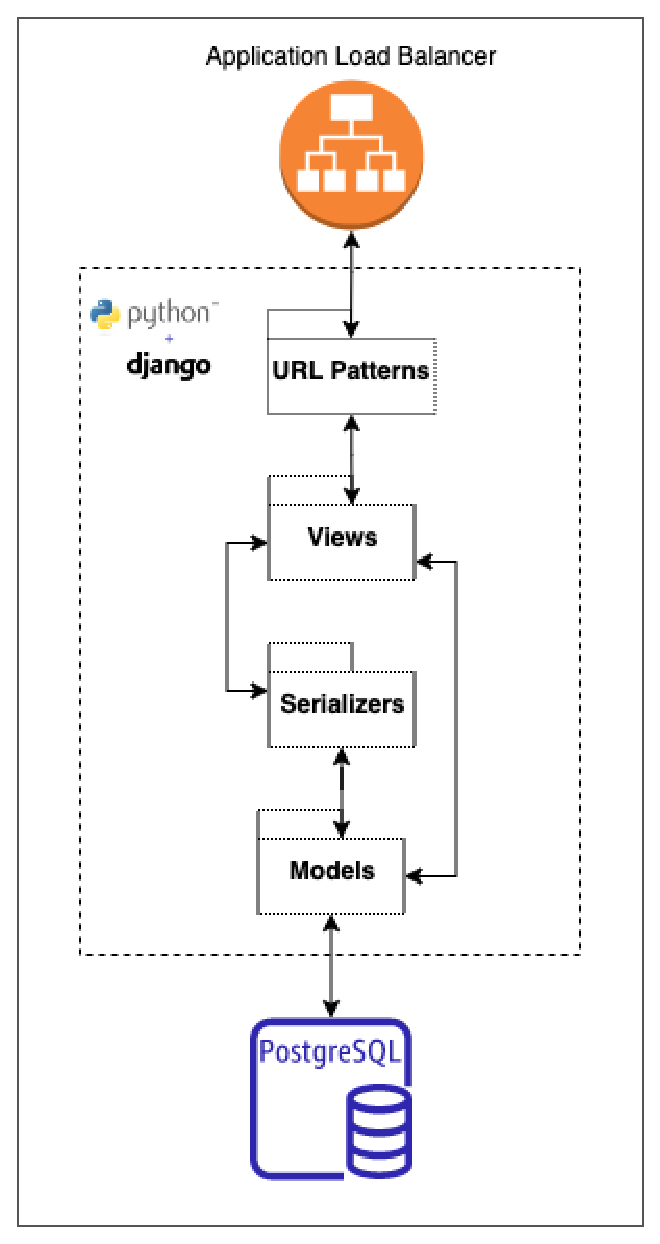
\includegraphics[keepaspectratio=true,scale=0.6]{figuras/backend_packages.eps}
    \legend{Fonte: Autores}
    \label{fig:backend_packages}
\end{figure}

\subsection{Cliente}

O cliente é responsável por enviar as requisições ao servidor e receber as respostas. O cliente é composto por um conjunto de módulos que são responsáveis por realizar as tarefas do sistema. Cada módulo é responsável por uma tarefa específica. Os pacotes e tecnologias utilizadas no cliente são:

\begin{itemize}
    \item \textbf{Routers}: são classes que são utilizadas para definir as rotas da aplicação. Através das rotas é renderizado o componente correto para cada rota.
    \item \textbf{Components}: são classes que são utilizadas para definir os componentes da aplicação. Os componentes possuem uma estrutura HTML e são responsáveis por renderizar a interface do usuário.
    \item \textbf{Containers}: são classes que são utilizadas para definir os containers da aplicação. Os containers possuem a lógicas de negócio da aplicação.
    \item \textbf{Services}: são classes que são utilizadas para definir os serviços da aplicação. Os serviços são responsáveis por realizar as requisições ao servidor.
    \item \textbf{TypeScript}: é uma linguagem de programação fracamente tipada. O TypeScript é uma linguagem de programação de código aberto e é uma das linguagens de programação mais utilizadas no mundo. O TypeScript é uma linguagem de programação que é transcompilada para JavaScript.
    \item \textbf{ReactJS}: é uma biblioteca JavaScript para criação de interfaces de usuário. O ReactJS é uma biblioteca de código aberto e é uma das bibliotecas JavaScript mais utilizadas no mundo.
\end{itemize}

\begin{figure}[h!]
    \centering
    \caption{Representação de pacotes e tecnologias do cliente}
    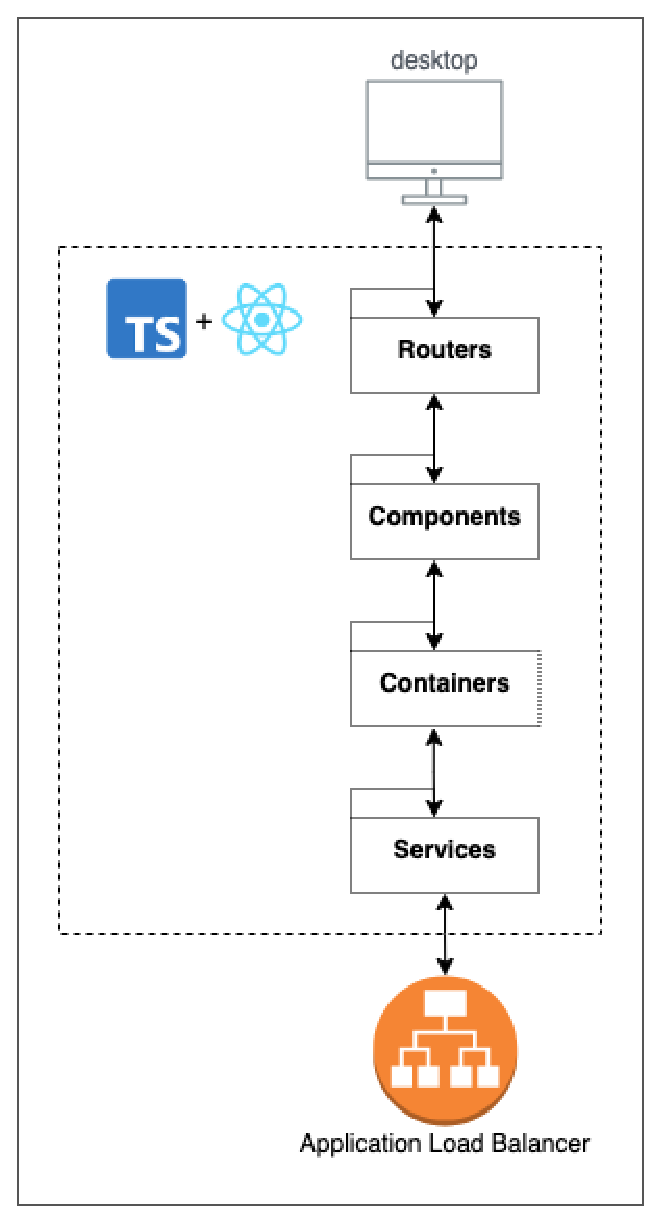
\includegraphics[keepaspectratio=true,scale=0.6]{figuras/frontend_packages.eps}
    \legend{Fonte: Autores}
    \label{fig:frontend_packages}
\end{figure}

\section{Modelo de Dados}

Um modelo de dados é uma representação abstrata de como os dados são estruturados e como eles se relacionam entre si. Ele é utilizado para descrever a estrutura lógica e conceitual dos dados, independentemente da forma como eles são armazenados ou implementados em um sistema. Existem vários tipos de modelos de dados, como o modelo relacional, o modelo de objeto-relacional e o modelo de dados NoSQL.

A escolha do modelo de dados é uma decisão importante, pois ela afeta diretamente a forma como os dados são armazenados e manipulados. O modelo de dados escolhido deve ser capaz de atender as necessidades do sistema. O modelo de dados escolhido para o sistema é o modelo relacional, pois ele é o modelo de dados mais utilizado no mundo e é capaz de atender as necessidades do sistema.

Abaixo é apresentado o modelo de dados do sistema. O modelo de dados é composto por 4 entidades: \textit{User}, \textit{Project}, \textit{Quizz} e \textit{Score}. Além das entidades, o modelo de dados é composto por 4 relacionamentos entre as entidades: \textit{SocialUser}, \textit{QuizzAnswer}, \textit{UserQuizzAnswer} e \textit{MonthlyScore}:

\begin{figure}[h!]
    \centering
    \caption{Modelo de dados do sistema}
    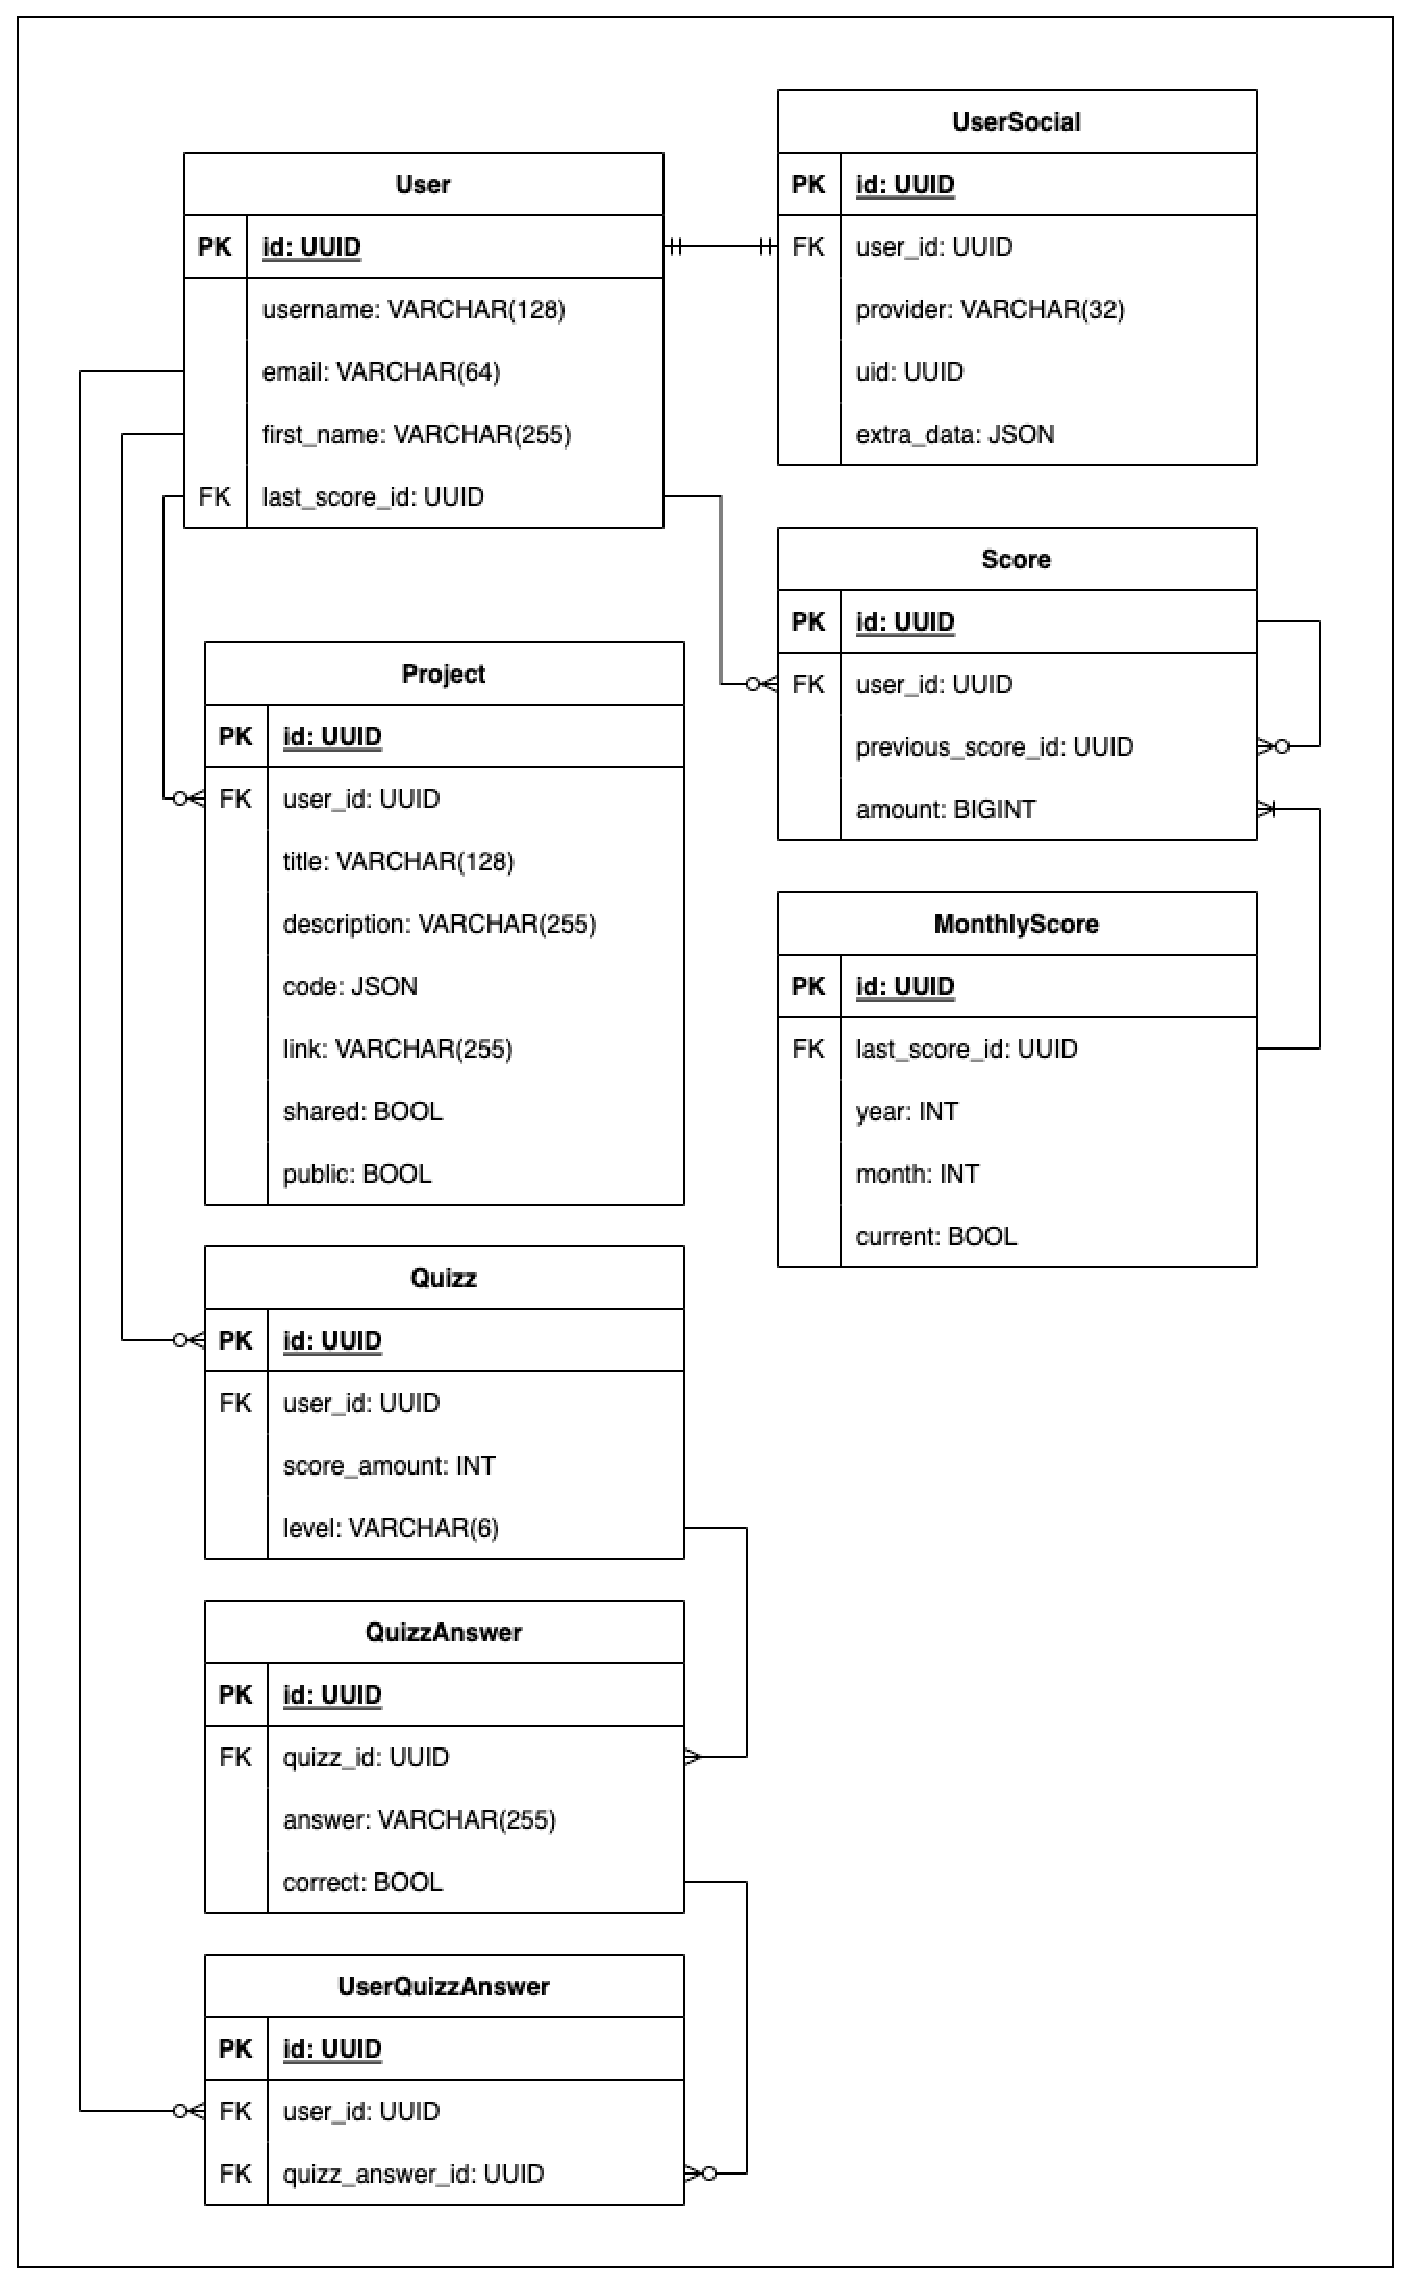
\includegraphics[keepaspectratio=true,scale=0.6]{figuras/modelo_de_dados.eps}
    \legend{Fonte: Autores}
    \label{fig:modelo_dados}
\end{figure}
